
%TeXstudio produce a LOT of warning yet still compile.

\documentclass[11pt]{beamer} 

\usetheme{metropolis} %https://github.com/matze/mtheme
\metroset{everytitleformat = regular,progressbar=foot} %settings
\mode<presentation>
%\usecolortheme{dove} %dove
% albatross, beaver, beetle, crane, default, dolphin, dove, orchid, rose, seagull, seahorse, whale, wolverine
%dont use  fly, lily,
%http://mirror.ox.ac.uk/sites/ctan.org/macros/latex/contrib/beamer/doc/beameruserguide.pdf
\setbeamercolor{title separator}{fg = UniBlue}
\setbeamercolor{frametitle}{fg = deepBlue, bg=aBlue!70}

\usepackage{booktabs}
\usepackage[scale=2]{ccicons}
\usepackage{pgfplots}
\usepgfplotslibrary{dateplot}
%\usepackage[demo]{graphicx}
\usepackage[font={small,it}]{caption}
\usepackage{subcaption} %throws a lot of errors but compile

%%LOGO
\usepackage{tikz}
\addtobeamertemplate{frametitle}{}{%
\begin{tikzpicture}[remember picture,overlay]
\node[anchor=north east,yshift=2pt] at (current page.north east) {
\includegraphics[height=0.8cm]{./../logo.png}};
\end{tikzpicture}}

%My std preamble for the docs
%\selectlanguage{british}%
\usepackage[british]{babel}
\usepackage{microtype} %better text
\IfFileExists{lmodern.sty}{\usepackage{lmodern}}{} %type 1 vector font
%
\usepackage{lettrine}
\usepackage{listings} %Add list support
\usepackage{colortbl} %colors in TABLES
%\usepackage{tikz,amsmath, amssymb,bm,color}
\usepackage{nicefrac}
\usepackage{lastpage} %get last page

%COLORS
\usepackage{color}
\definecolor{lightgray}{gray}{0.8} %for colortbl
\definecolor{UniBlue}{RGB}{83,121,170}
\definecolor{deepBlue}{HTML}{000066}
\definecolor{blueBgd}{HTML}{99C8FF}
\definecolor{aBlue}{HTML}{1879F7}

%%%%%%%%%%%%%%%%%%%%%%%%%%%%%%%%%%%%%%%%%%%%%%%%%%%%%%%%%%%%%%%%%%
%FOOTNOTES
%nice look after http://www.dedoimedo.com


%%%%%%%%%%%%%%%%%%%%%%%%%%%%%%%%%%%%%%%%%%%%%%%%%%%%%%%%%%%%%%%%%%%
%TABLE SETTINGS
\usepackage{colortbl} %colors in table
\usepackage{rotating} %rotatins within tables
\usepackage{multirow}
\renewcommand{\arraystretch}{1.2} %add padding/spacing
%\usepackage{adjustbox}%rotating and fitting into page
%

\usepackage{booktabs} % To thicken table lines
%define thickness of table lines
\let\mytoprule\toprule
\renewcommand{\toprule}{\mytoprule[0.20em]}
\let\mytoprule\bottomrule
\renewcommand{\bottomrule}{\mytoprule[0.20em]}
\let\mytoprule\midrule
\renewcommand{\midrule}{\mytoprule[0.08em]}

\usepackage{spreadtab} % for simple calculations

%vertically and horizontally centered multicolumn cells with a fixed width. M{width}
%\newcolumntype{M}[1]{>{\centering\hspace{0pt}}m{#1}}
% each spanned cell has the same width. S{width of multicolumn cell}{number of spanned columns}
%\newcolumntype{S}[2]{>{\centering\hspace{0pt}}m{(#1+(2\tabcolsep+\arrayrulewidth)*(1-#2))/#2}}

%%%%%%%%%%%%%%%%%%%%%%%%%%%%%%%%%%%%%%%%%%%%%%%%%%%%%%%%%%%%%%%%%%%
%TikZ
\usepackage{tikz}

\colorlet{red}{red!50}
\colorlet{green}{green!50}
\colorlet{blue}{blue!50}
\definecolor{yellow}{HTML}{FFFF00}
\colorlet{yellow}{yellow!50}
\definecolor{fiolet}{HTML}{7030A0}
\colorlet{fiolet}{fiolet!50}
\colorlet{bgd_main}{black!50}
\colorlet{bgd}{bgd_main!75}
\colorlet{bgd2}{bgd_main!50}
\colorlet{bgd3}{bgd_main!25}
\colorlet{bgd4}{bgd_main!15}

\usetikzlibrary{shapes,arrows,calc,positioning}

%%%%%%%%%%%%%%%%%%%%%%%%%%%%%%%%%%%%%%%%%%%%%%%%%%%%%%%%%%%%%%%%%%%
% Footnotes in Figs
%\rule[raise-height]{width}{thickness}
\newcommand*{\FigFootnote}[1]{
\noindent \begin{flushleft}
\rule[0.2ex]{0.4\columnwidth}{0.5pt}
\par
\footnotesize
#1
\footnotesize
\end{flushleft}
}

%%%%%%%%%%%%%%%%%%%%%%%%%%%%%%%%%%%%%%%%%%%%%%%%%%%%%%%%%%%%%%%%%%%
%MATH, number display
%need to install siunitx, l3kernel,l3packages
\usepackage{siunitx} %this is for units display

\sisetup{per-mode=fraction, tight-spacing = true , fraction-function = \nicefrac, quotient-mode = fraction}% %nicefrac \tfrac
\sisetup{inter-unit-product = \ensuremath { { } \cdot { } } , exponent-product = \cdot }%
\sisetup{input-product=x , output-quotient =  \ensuremath { { } \times{}}} %for 1x2x3
%number grouping(3), std==true %\sisetup{group-digits = decimal} 
\sisetup{group-minimum-digits = 4} %start grouping from 4 digits, in 3 no groups
\sisetup{range-units = single,range-phrase = \,--\,} %2-3C not 2C-3C %, range-phrase = --
\sisetup{separate-uncertainty=true} %2+-1 not 2(1)
\sisetup{prefixes-as-symbols=true } % , scientific-notation = engineering false for 10^-9 ect ect , exp in multiple of 3
\sisetup{range-phrase = \,-\, } % , refo of ranges
%\sisetup{zero-decimal-to-integer, round-mode = places,round-precision = 3}
%\sisetup{add-arc-degree-zero=true , add-arc-minute-zero=true ,add-arc-second-zero=true} %for angle settings

%This is to auto convert ns,ms,us to 10^-xx s
\DeclareSIUnit[scientific-notation = engineering, prefixes-as-symbols=false]{\psec}{\pico\second}
\DeclareSIUnit[scientific-notation = engineering, prefixes-as-symbols=false]{\nsec}{\nano\second} 
\DeclareSIUnit[scientific-notation = engineering, prefixes-as-symbols=false]{\usec}{\micro\second}
\DeclareSIUnit[scientific-notation = engineering, prefixes-as-symbols=false]{\msec}{\milli\second} 

%...AND SOME UNITS
\DeclareSIUnit\dBm{dBm}
\DeclareSIUnit\ppm{ppm} %{\num{1e-6}}%{ppm}
\DeclareSIUnit\yr{yr} %{{361}\day}<-nice nice
\DeclareSIUnit\cy{cycle} %phase cycle
\DeclareSIUnit\epoch{epoch} %GPS/LL epoch
\DeclareSIUnit\inch{"} %inch 
\DeclareSIUnit\wk{week} %week
\DeclareSIUnit\hr{hrs} %hours
\DeclareSIUnit\min{minute} %hours
\DeclareSIUnit\mile{mi}
\DeclareSIUnit\Mcps{Mcps}
\DeclareSIUnit\bit{bit}
\DeclareSIUnit\chip{chip length}
%Other units
\newcommand*{\GBP}[1]{$\SI{#1}[\textsterling]{}$}


%%%%%SHORTHANDS (Standard Sentences)
%\newcommand*{\Myrange}[3]{$\textrm{\SIrange{#1}{#2}{#3}}$}


%how much work per week
\newcommand*{\wkWrk}[1]{$\SI{#1}{\hr\per\wk}$}

%references
\newcommand*{\tabref}[1]{shown in table \ref{#1} on page \pageref{#1}\xspace}
\newcommand*{\vref}[1]{\ref{#1} on page \pageref{#1}\xspace}


%\renewcommand{\baselinestretch}{1.2} %line spacing
%{\setstretch{1.0}\color{blue} text bla bla } for section strech
\renewcommand{\footnotesize}{\scriptsize} %change footnote sizes
\newcommand{\thisDocRef}{\footnote{History of changes at \url{https://github.com/DfAC/TeachingSlides/}.}}
%\usepackage{lipsum} % for dummy text only

%Grey text
\definecolor{shadecolor}{RGB}{190,190,190}
%\textcolor{shadecolor}{	\item[Ogaja\_Matlab.7z] Matlab script. To be placed on-line after week2.}


%%%%%%%%%%%%%%%%%%%%%%%%%%%%%%%%%%%%%%%%%%%%%%%%%%%%%%%%%%%%%%%%%%%%%%%%%%%%%%
%%%%%%%%%%%%%%%%%%%%%%%%%%%%%%%%%%%%%%%%%%%%%%%%%%%%%%%%%%%%%%%%%%%%%%%%%%%%%%
\title[H24VEP]{H24VEP Project 3}
\subtitle{Bridge Monitoring Preparation\thisDocRef}

\author{LKB/SI\footnote{Based on presentation given by the last year MSc cohort. All Google Map screen-shots have been attributed as per guideline. All graphics copyrights belongs to their respective owners.\\}}
%\newline to prevent footnote cut off, otherwise use \hskip1.2cm
\institute{NGI}
\date{\today}

\begin{document}
	
	\begin{frame}
		\titlepage
	\end{frame}
	
	% Uncomment these lines for an automatically generated outline.
	\begin{frame}{Outline}
		\tableofcontents
	\end{frame}
	
\section{Introduction}

\begin{frame}[allowframebreaks]{Project Introduction}

The aim of the project is to characterise bridge movement using precise geodetic sensors. We will monitor Wilford Pedestrian Bridge Monitoring Using GNSS, Robotic Total Station (RTS), IMU and Inclinometer sensors. We will also try to excite the structure to better understand sensors performance and to characterise bridge movement.

To do so we will:

\begin{itemize}
	\item Decide where do put sensors on the bridge;
	\item Decide how are you going to do it;
	\item Analyse measurements from multiple sensors;
	\item Examine the bridge's response under different excitation types;
	\item Compare and contrast the results;
	\item Tell the story.
\end{itemize}
\end{frame}

\begin{frame}{Wilford Pedestrian Bridge}
Wilford Pedestrian Bridge is single span suspension bridge. Spans the River Trent; 69 m long and 3.7 m wide.
	%\begin{center}
	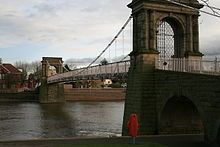
\includegraphics[width=.6\textwidth]{pic/Bridge01.jpg}
	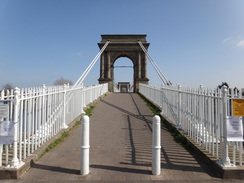
\includegraphics[width=.55\textwidth]{pic/Bridge02.jpg} 
	\captionof{figure}{Wilford Pedestrian Bridge} %to make images on top of each other
	%\end{center}
	%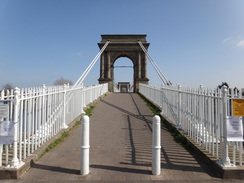
\includegraphics[width=.4\textwidth]{pic/Bridge02.jpg} 

\end{frame}

\begin{frame}{Equipment}

We plan to use following equipment on the bridge:

\begin{itemize}
	\item Leica GNSS receiver x5
	\item Leica Robotic Total Station (RTS) x2
	\item Novatel SPAN IMU sensor x1
	\item Leica Nivel 210 inclinometer x1
\end{itemize}

\end{frame}


% Time scale
% bridge location

\begin{frame}{Plan}%{Daily repetition}
\begin{itemize}
	\item What equipment are you using? 
	\item Where are you placing it?
	\item	How are you going to time synchronise equipment?
	\item What about coordinate system?
	\item How many ppl you have?
	\item Who is responsible for what?
	\item How can we prevent mistakes? How can we prevent accidents?
\end{itemize}
\end{frame}

\begin{frame}{H\&S}%{Daily repetition}
\begin{center}
	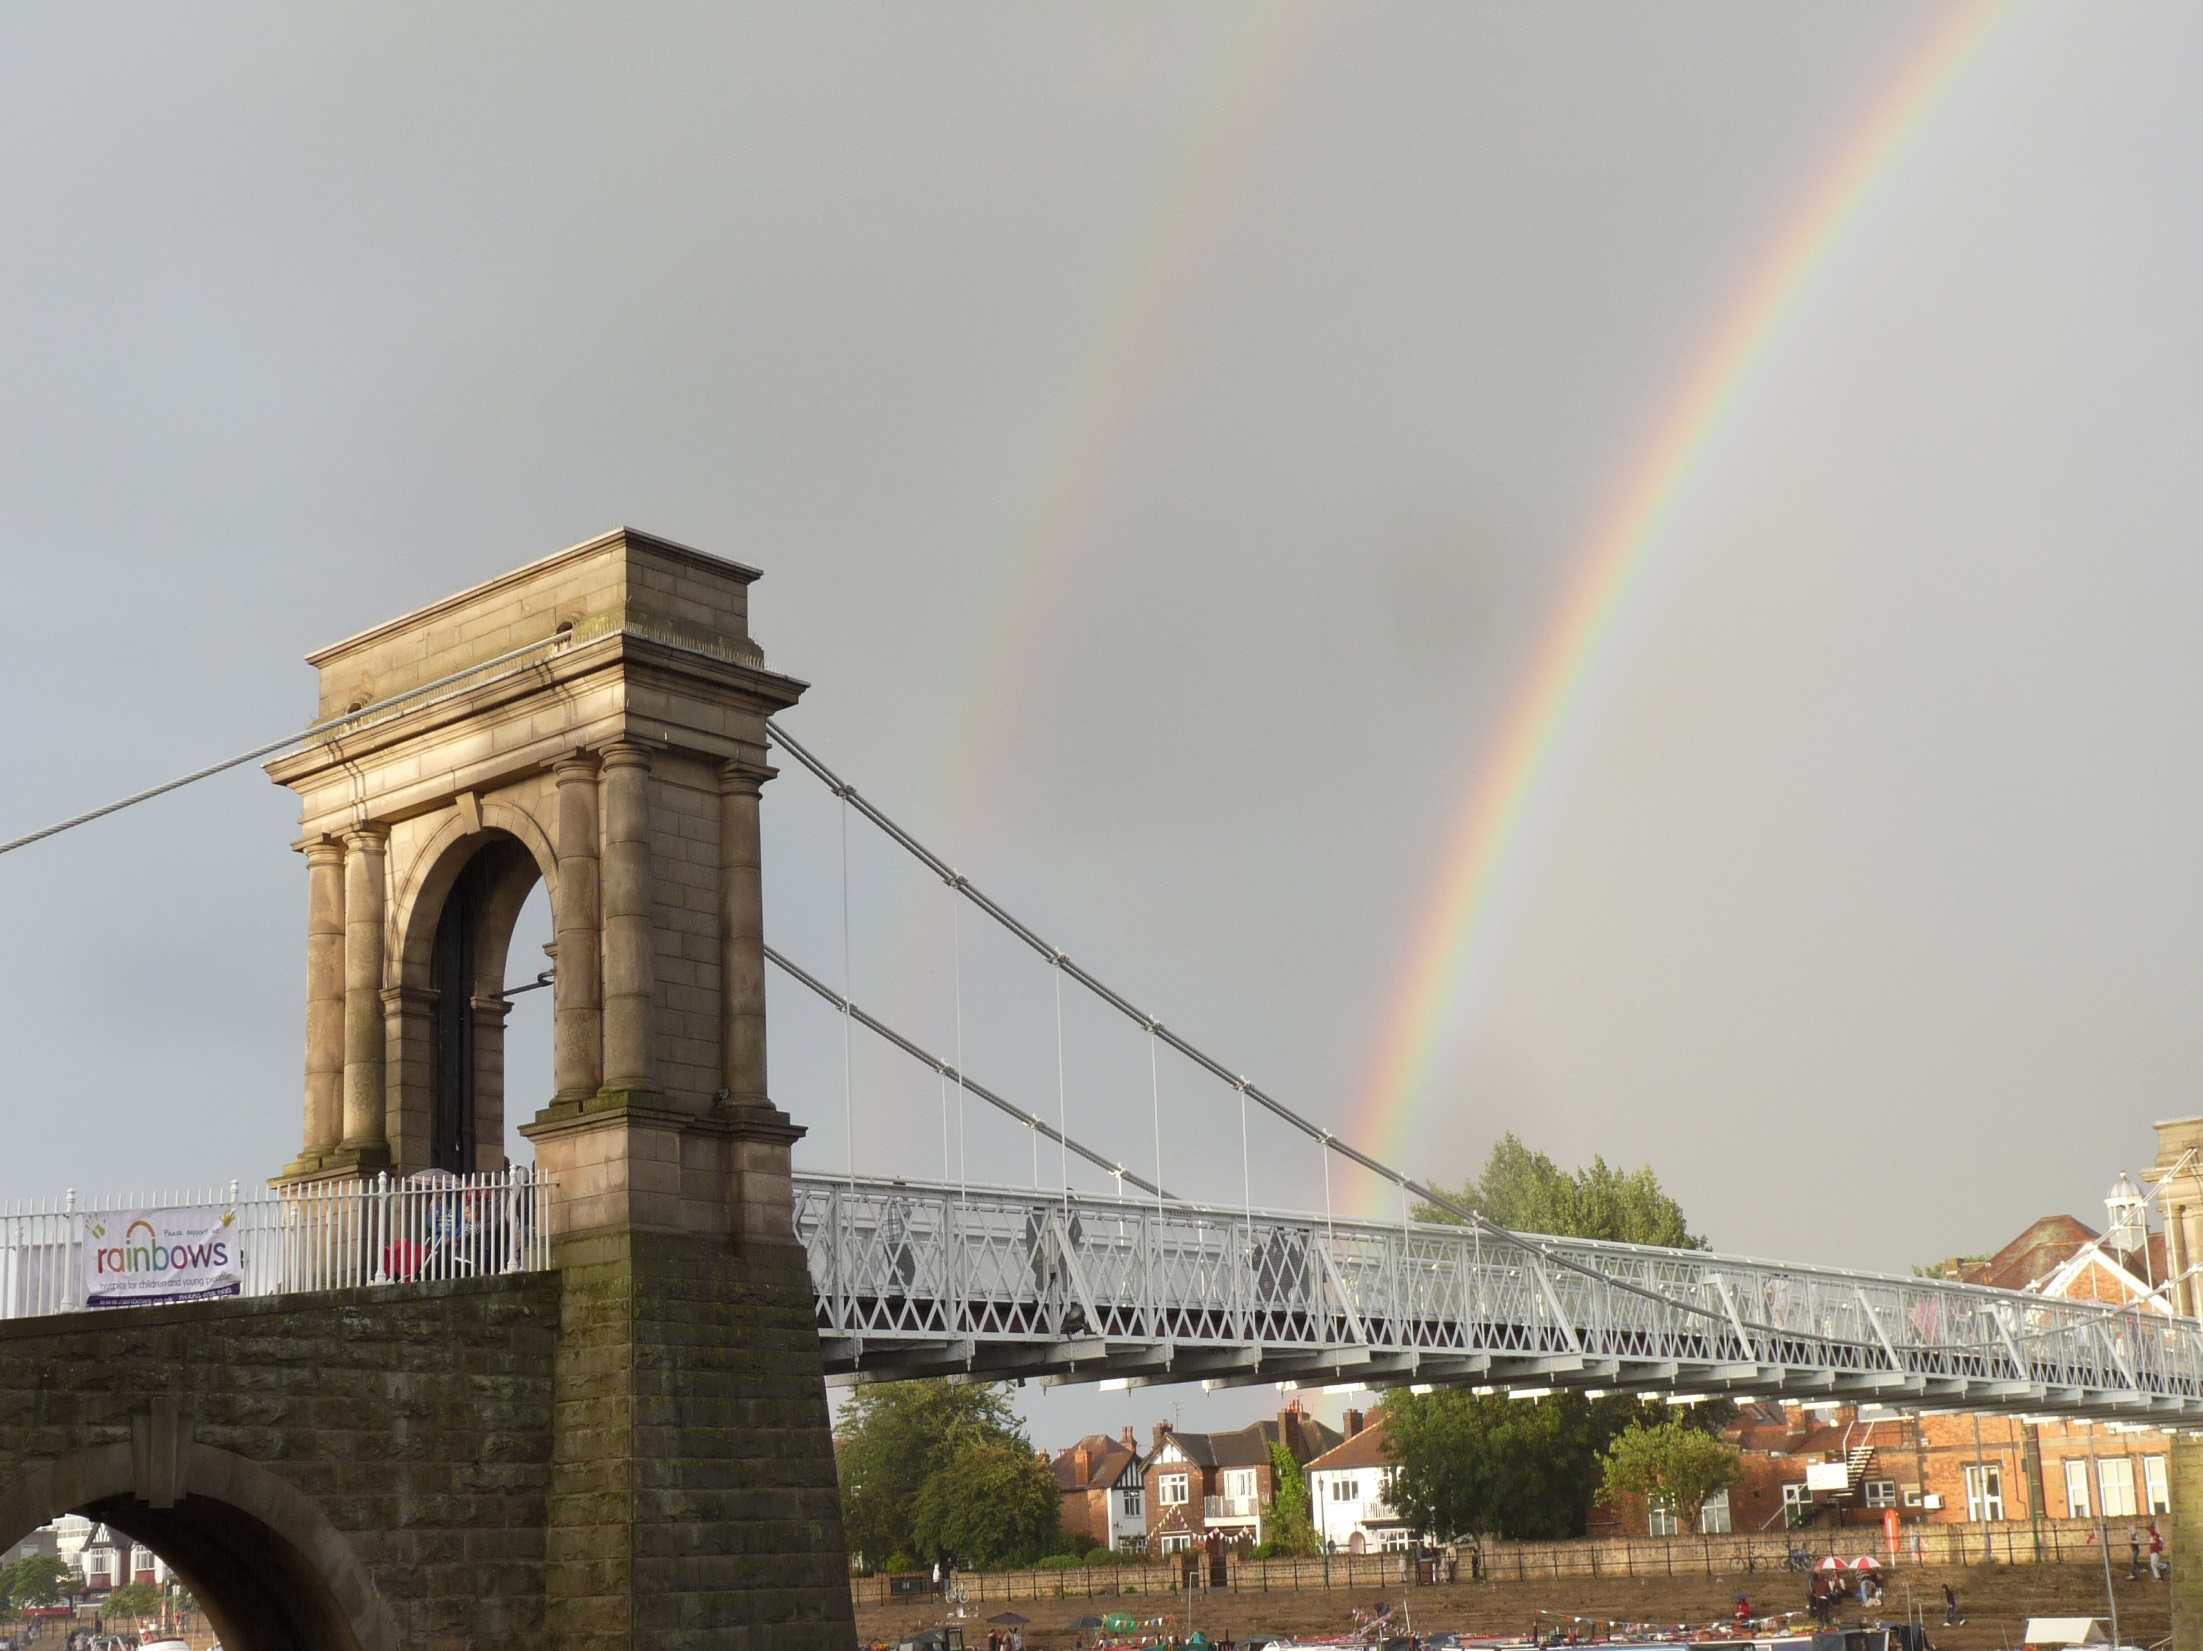
\includegraphics[width=.8\textwidth]{pic/rainbow.jpg}
	\captionof{figure}{Have you got risk assessment?} %to make images on top of each other
\end{center}
\end{frame}


\section{Implementation}

\begin{frame}{Bridge layout}%{Daily repetition}
	\begin{center}
	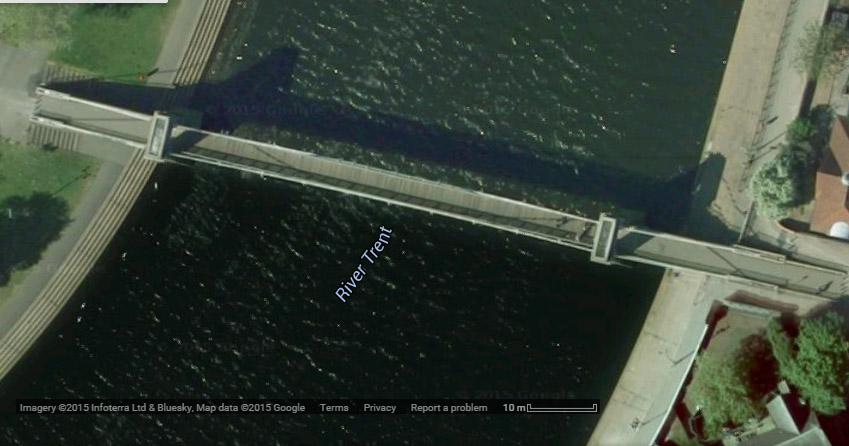
\includegraphics[height=.6\textheight]{pic/BridgeBare.jpg}
	\captionof{figure}{Top view} %to make images on top of each other
	\end{center}
\end{frame}

\begin{frame}{Sensors layout}%{Daily repetition}
	\centering
	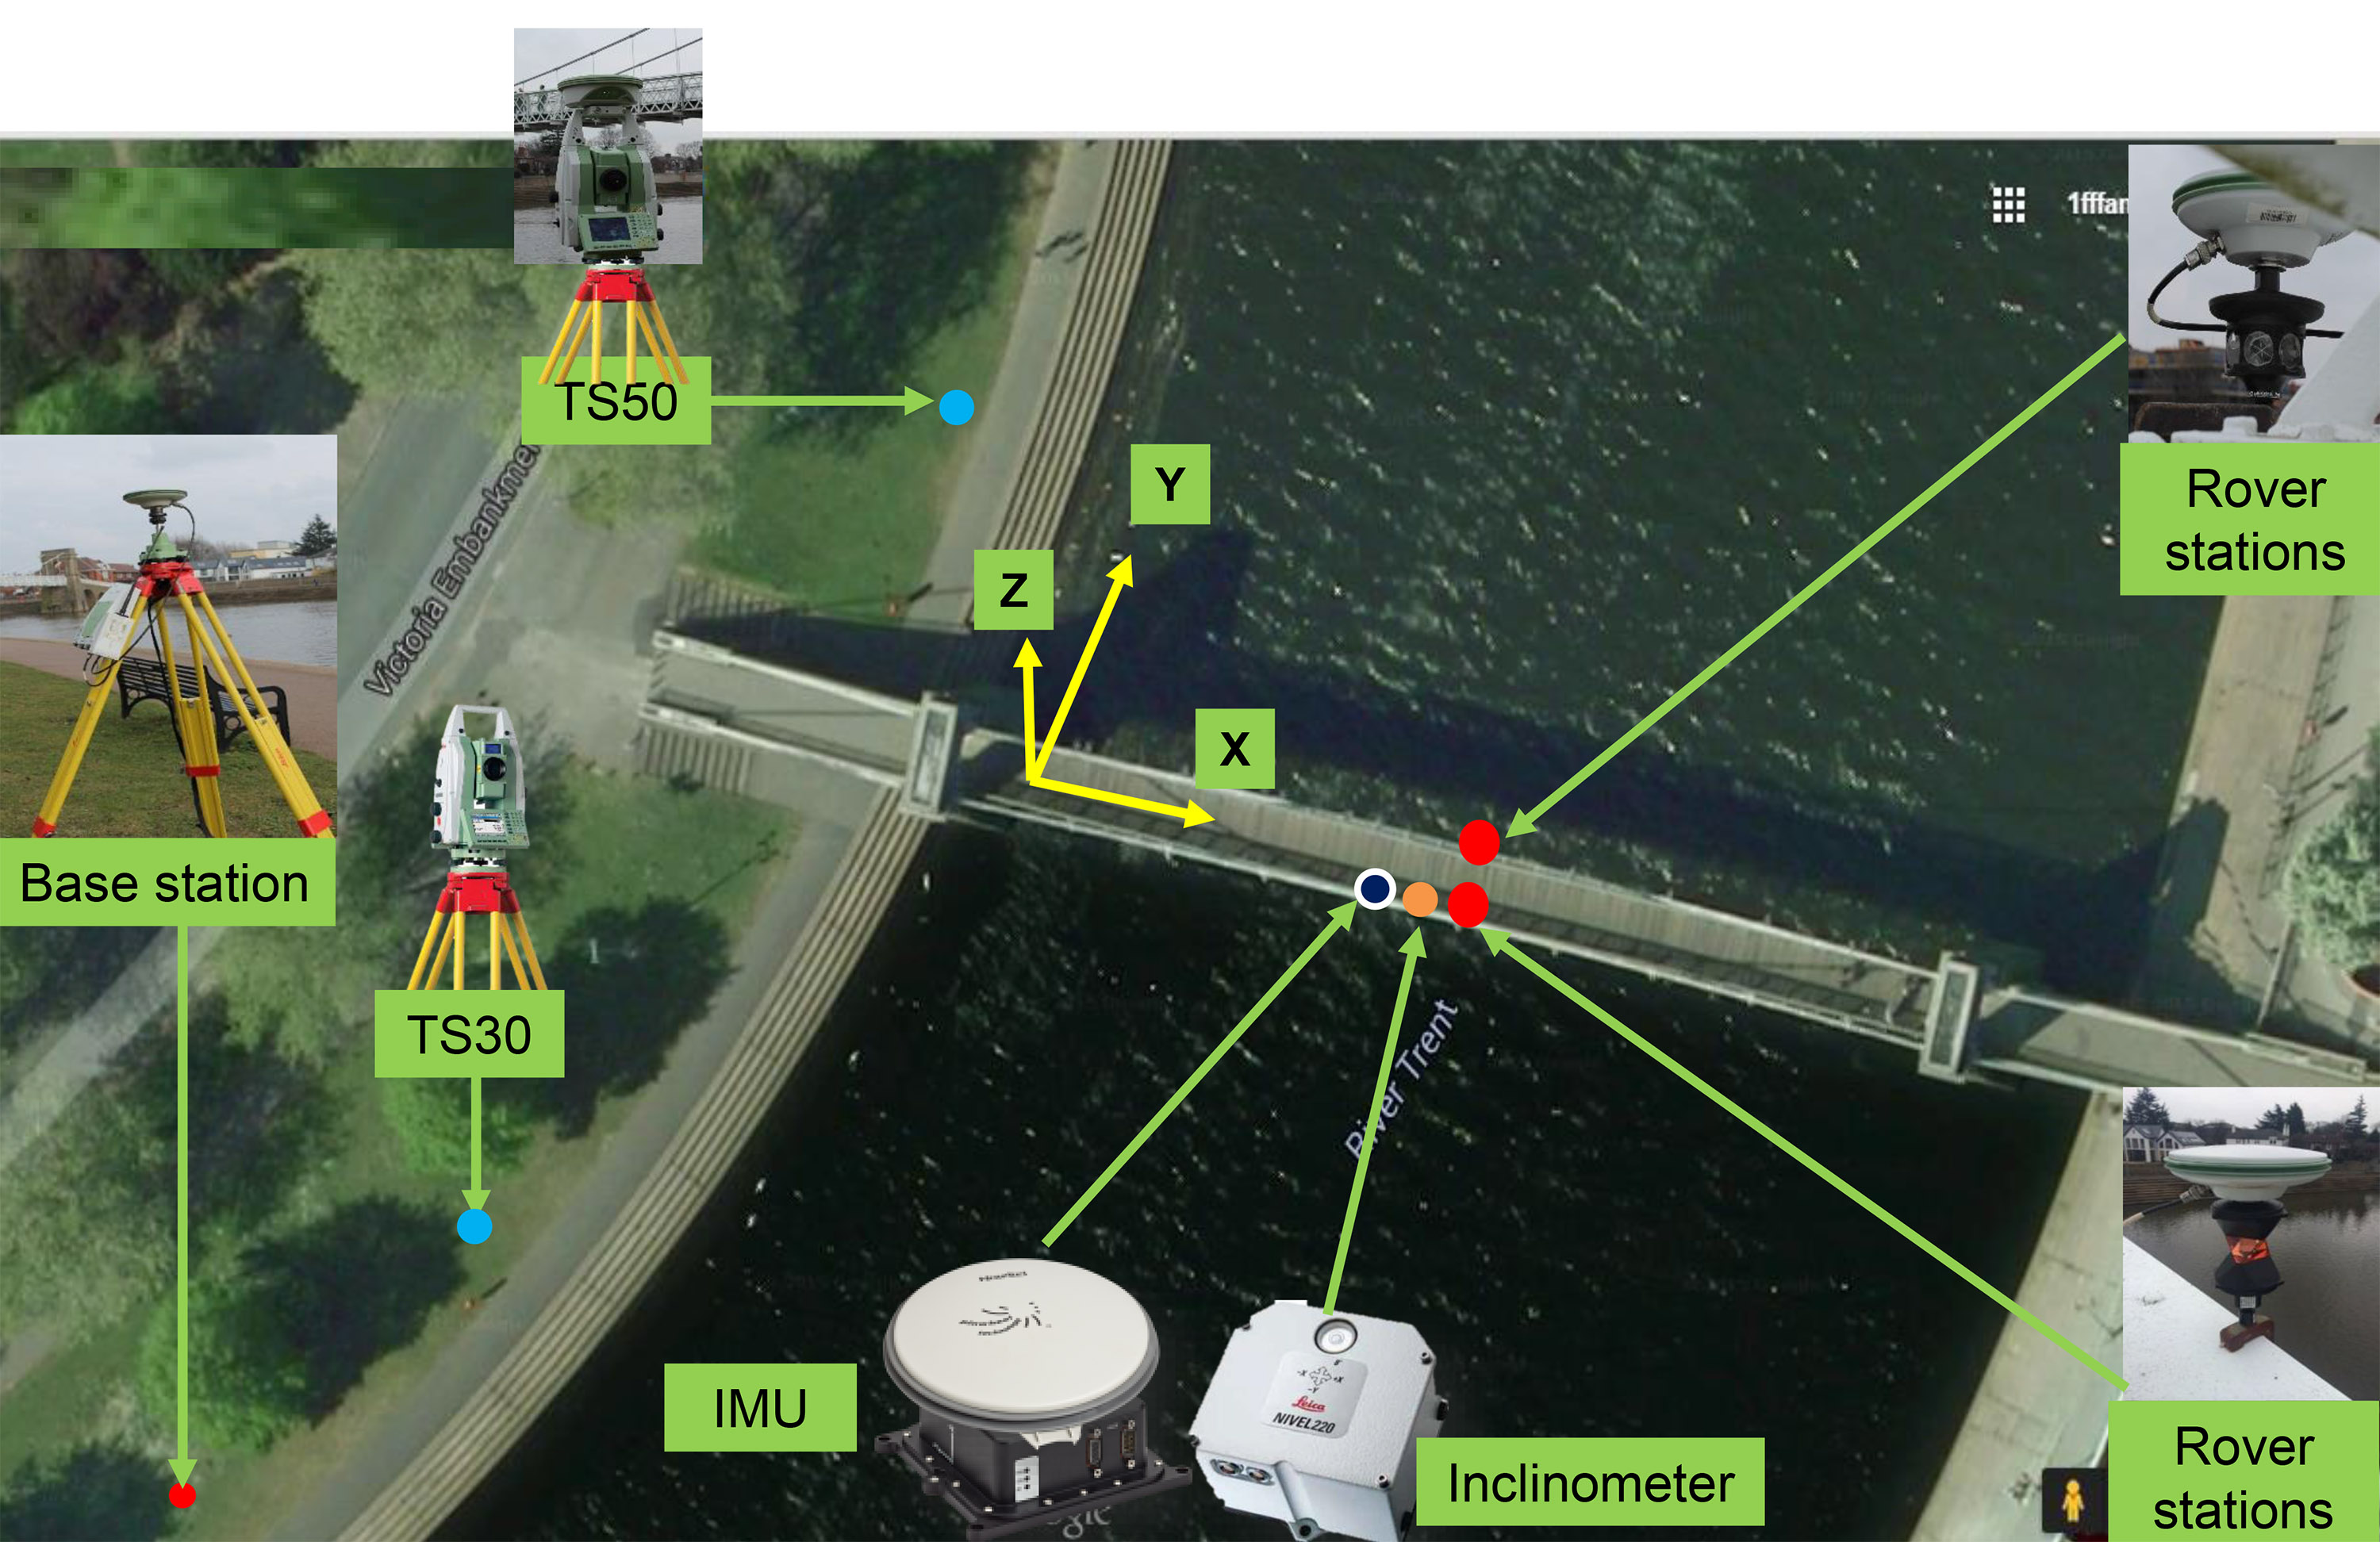
\includegraphics[height=.7\textheight]{pic/layout.jpg}
	\captionof{figure}{Location of the sensors from last year} %to make images on top of each other

\end{frame}

\begin{frame}{Excitation}%{Daily repetition}
	To better understand sensors performance and to characterise bridge movement we will also create artificial excitation of the bridge.

	\centering
	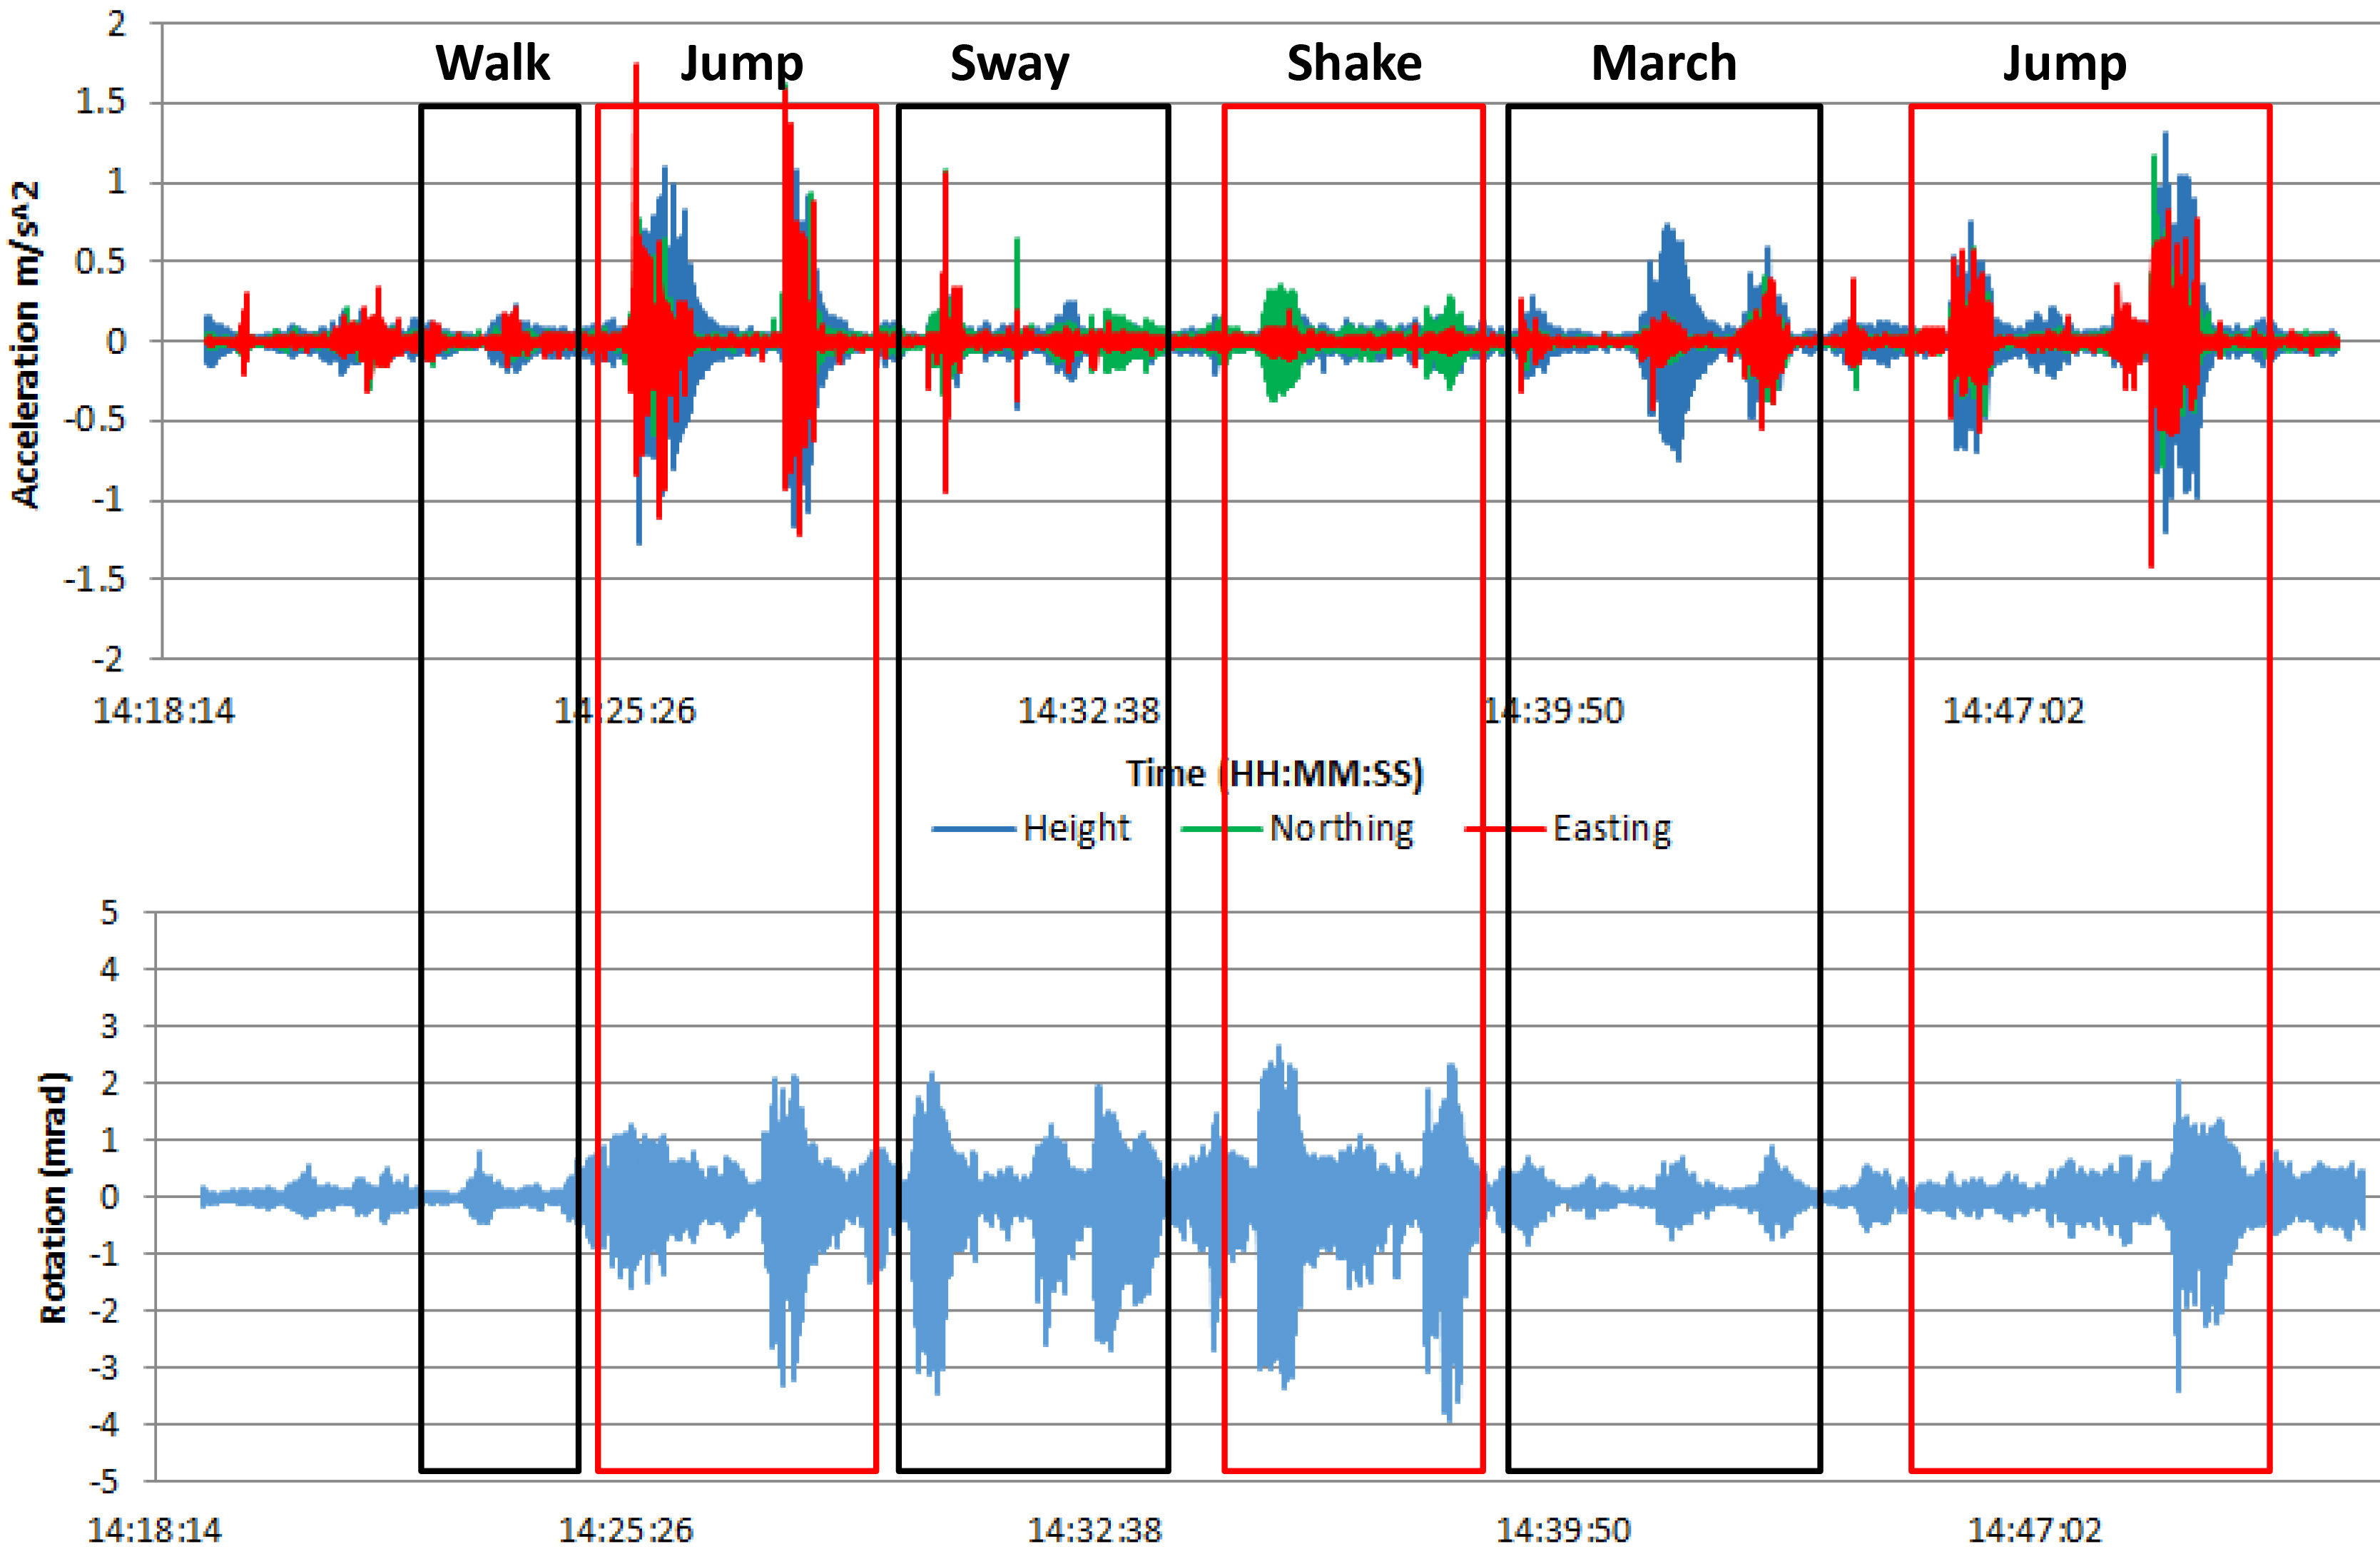
\includegraphics[height=.6\textheight]{pic/excitation.jpg}
	\captionof{figure}{Example of excitations from last year trial} %to make images on top of each other
	%\captionof{figure}{Example of visualisation}
\end{frame}


\section{Summary}


	\begin{frame}{Summary}
	\begin{itemize}
		\item Decide on your equipment.
		\item Decide on your activities.
		\item Select Time Keeper and Note Keeper.
		\item Agree on roles (responsibilities) before next Monday.
		\item Submit all relevant H\&S forms before Thursday.
	\end{itemize}
	\end{frame}


%Final slide
\setbeamercolor{background canvas}{bg=blueBgd!60}
\plain{Good luck\thisDocRef}

\end{document}
